
%% bare_conf.tex
%% V1.4b
%% 2015/08/26
%% by Michael Shell
%% See:
%% http://www.michaelshell.org/
%% for current contact information.
%%
%% This is a skeleton file demonstrating the use of IEEEtran.cls
%% (requires IEEEtran.cls version 1.8b or later) with an IEEE
%% conference paper.
%%
%% Support sites:
%% http://www.michaelshell.org/tex/ieeetran/
%% http://www.ctan.org/pkg/ieeetran
%% and
%% http://www.ieee.org/

%%*************************************************************************
%% Legal Notice:
%% This code is offered as-is without any warranty either expressed or
%% implied; without even the implied warranty of MERCHANTABILITY or
%% FITNESS FOR A PARTICULAR PURPOSE! 
%% User assumes all risk.
%% In no event shall the IEEE or any contributor to this code be liable for
%% any damages or losses, including, but not limited to, incidental,
%% consequential, or any other damages, resulting from the use or misuse
%% of any information contained here.
%%
%% All comments are the opinions of their respective authors and are not
%% necessarily endorsed by the IEEE.
%%
%% This work is distributed under the LaTeX Project Public License (LPPL)
%% ( http://www.latex-project.org/ ) version 1.3, and may be freely used,
%% distributed and modified. A copy of the LPPL, version 1.3, is included
%% in the base LaTeX documentation of all distributions of LaTeX released
%% 2003/12/01 or later.
%% Retain all contribution notices and credits.
%% ** Modified files should be clearly indicated as such, including  **
%% ** renaming them and changing author support contact information. **
%%*************************************************************************


% *** Authors should verify (and, if needed, correct) their LaTeX system  ***
% *** with the testflow diagnostic prior to trusting their LaTeX platform ***
% *** with production work. The IEEE's font choices and paper sizes can   ***
% *** trigger bugs that do not appear when using other class files.       ***                          ***
% The testflow support page is at:
% http://www.michaelshell.org/tex/testflow/



\documentclass[conference]{IEEEtran}
% Some Computer Society conferences also require the compsoc mode option,
% but others use the standard conference format.
%
% If IEEEtran.cls has not been installed into the LaTeX system files,
% manually specify the path to it like:
% \documentclass[conference]{../sty/IEEEtran}
\usepackage[utf8]{inputenc}
\usepackage[pdftex]{graphicx}
\graphicspath{{Images/}}
\DeclareGraphicsExtensions{.pdf,.png,.jpg}
% correct bad hyphenation here
\hyphenation{op-tical net-works semi-conduc-tor}

\begin{document}
%
% paper title
% Titles are generally capitalized except for words such as a, an, and, as,
% at, but, by, for, in, nor, of, on, or, the, to and up, which are usually
% not capitalized unless they are the first or last word of the title.
% Linebreaks \\ can be used within to get better formatting as desired.
% Do not put math or special symbols in the title.
\title{Vad är en bra projektmetod för små IT-projekt?}


% author names and affiliations
% use a multiple column layout for up to three different
% affiliations
\author
    {
      \IEEEauthorblockN{Sebastian Heimlén\textsuperscript{1},
        Henrik Björklund\textsuperscript{2},
        Yobart Amino\textsuperscript{3},
        Teo Klestrup Röijezon\textsuperscript{4}}
        \IEEEauthorblockA{\textit{KTH Royal Institute of Technology}
          \textit{Isafjordsgatan 22, 164 40 Kista, Sweden}\\
          \texttt{\textsuperscript{1}heimlen@kth.se}\\
          \texttt{\textsuperscript{2}hebjo@kth.se}\\
          \texttt{\textsuperscript{3}yobart@kth.se}\\
          \texttt{\textsuperscript{4}teo@nullable.se}
         } 
    }

% make the title area
\maketitle

% As a general rule, do not put math, special symbols or citations
% in the abstract
\begin{abstract}
  this is an abstract.

  \textbf{\textit{keywords} - with keywords}
\end{abstract}

\IEEEpeerreviewmaketitle

\section{Om detta dokument och undersökning}
Detta dokument är en del av examen i kursen ''Projekt och projektmetoder'' och skall förmedla känslor, tankar och slutsatser vilket vår projektgrupp förvärvat under  projektarbete i denna kurs. Detta dokument kommer att läsas av kursens examinator och utvärderas enligt ''Blooms taxonomi''
, en stor del av detta dokument skrivs gemensamt av gruppens medlemmar, medan vissa specifika delar skrivs av enskilda medlemmar baserat på den projektroll de antagit under projektet. Vilket som ett exempel kan ges att sudenten som hade rollen som projektledare att skriva om sina erfarenheter och slutsatser inom den rollen.

Detta dokuments trovärdighet anses vara hög, då innehållet är baserat på våra egna erfarenheter och upplevelser från att ha genomfört detta projekt, vars projektmetoder bygger på erkända och välanvända projektmetoder inom just IT-projekt och produkt-utveckling. Dokumentet innehåller också referenser till  erkända böcker, tidsskrifer samt vetenskapliga texter inom projektmetoder, vilket ger arbetet en hög trovädighetsfaktor.
\section{Introduktion}

%\hfill mds
 
%\hfill August 26, 2015

\subsection{Bakgrund}
Detta är en rapport som skrivs i samband med kursen ''Projekt och projektmetoder'' i vilket studenter i små grupper genomför ett IT-projekt i syfte att pröva på samt analysera olika projektmetoder, dessa analyser ska sedan diskuteras och framföras i denna rapport för att kunna besvara frågeställningen ''Vad är en bra projektmetod för små IT-projekt''. För att besvara denna frågeställning ska studenterna i sina projektgrupper skapa en produkt som innefattar både hårdvara, mjukvara, datornätverk samt elektronik.\\
\\
Kursens syfte är att fördjupa studenternas kunskap inom projektmetodik och skall fungera som en förberedelse inför både examensarbete samt det fortsatta arbetslivet efter examen. Kursen projektgrupper består av både data- samt elektrostudenter, och tanken bakom detta är att studenter från de olika programmen har olika expertisområden, vilket leder till att olika studenter har olika ansvarsområden inom projektgruppen, ett mål med kursen är att projektgruppen tillsammans ska utvecklas och dela med sig av sin kunskap, vilket leder till att samtliga medlemmar ytterliggare utvecklas på en personlig nivå.

\subsection{Problemformulering}
Den övergripande frågeställningen är som tidigare nämnt ''Vad är en bra projektmetod för små IT-projekt?'',  för att besvara denna frågeställning måste gruppen först undersöka samt komma överens om vad en bra projektmetod är. En bra utgångspunkt för att beskriva en bra projektmetod är projekt-triangel.En bra projektmetod kan ses som en metod där projektgruppen på ett strukturerat och planerat vis tar fram en produkt som tillfredställer kundens krav, och på samma gång utvecklar projektgruppens effektivitet och sammarbetsförmåga. En bra projektmetod innefattar hjälpmedel som underlättar och förbättrar arbetsgången och tillåter projektgruppen att snabbt och ofta ändra arbetssätt, arbetsbörda och/eller resultatet av projektarbetet. Detta är grundkraven för en bra projektmetod och det är därför som agila och iterativa projektmetoder är så populära inom IT-projekt. IT-projekt, och specifikt projekt som innefattar mjukvaru-utveckling är speciella, då det är lätt att projektgruppen skapar något som inte alls överensstämmer med vad kundens vision var. Det är därför viktigt att ofta återkoppla till kunden och snabbt kunna byta riktning i de fall där kunden känner att projektgruppen gått fel. Sommerville beskriver ett enligt honom bra arbetssätt för att genomföra IT-projekt i sin bok \textit{Software Engineering}\cite{Sommerville10} som innefattar fyra olika steg:\\
\\
1. Produktspecifikation, där projektgruppen tillsammans med kunden kommer överens om vilka krav och specifikationer som finns på produkten som ska tas fram.\\
\\
2. Produktframtagning, där projektgruppen designar och jobbar för att ta fram en produkt.\\
\\
3. Produktvalidering, där produkten blir testad och validerad för att försäkra att produkten uppfyller kraven.\\
\\
4. Produktutveckling, där projektgruppen ändrar produkten beroende på eventuella önskemål från kund.\\
\\
Dessa fyra steg skall göras i små iterationer så att en prototyp av produkten produceras snabbt, kan valideras och testas och samtal kan hållas med kunden för att se till att projektgruppen är på rätt spår, och i de fall kunden känner att projektgruppen har tänkt fel eller kommer på fler krav och/eller funktioner så kan projektgruppen snabbt börja utveckla och testa för dessa nya önskemål.

\subsection{Undersökningsstrategi/lösningsstrategi}
Strategien för att undersöka och hitta svar till denna frågeställning har varit att genomföra en fallstudie i vilken projektgruppen har genomfört ett projekt som har lett till en slutprodukt som levererats till kund. I detta projekt har projektgruppen testat ett antal olika projektmetoder, som samtliga medlemmar i gruppen tillsammans genom diskussion har beslutat att undersöka närmare, dessa projektmetoder har sedan diskuterats, analyserats och slutsatser har dragits, och dessa slutsatser kommer förmedlas i detta dokument.

\subsection{Avgränsningar}
Teorierna i denna rapport avgränsas genom att endast vissa förvalda projektmetoder tas upp, samt relativa teorier om dessa metoder. Dessa teorier begränsas till stor del av givna artiklar och dokument med viss komplimenterande dokument. IT miljö, studiemiljö, studenter, ett enda projektuppdrag. 

\section{Teori och ingenjörspraxis}
I detta avsnitt går teori som kommer att användas i detta projekt igenom, samt den ingengjörspraxis som brukas. Teorierna avhandlar teorier om projektmetoder, hur en grupp och dess individer arbetar i ett projekt, samt teorier om gruppdynamik.

\subsection{Teori}
Detta kapitel listar och i viss mån beskriver teorier och ingenjörspraxis som använts i undersökningen. Det finns två underkapitel, Litteraturstudie och Förstudie.
\subsection{Litteraturstudie}
I genomförandet av denna fallstudie har flera källor konsulterats, och i denna del ämnar vi att kortfattat beskriva dessa. Förutom de källor som anges finns förmodligen andra, och möjligtvis bättre, källor som ej konsulterats.\\
\\

\textbf{Övergripande källor för hela projektet}\\
\\
\textit{Software Engineering} av Ian Sommerville\cite{Sommerville10}. Denna bok behandlar främst IT-projekt inom mjukvaru-utveckling, men den tar även upp saker som är viktiga att ta med sig i vilket projekt som helst, denna bok är en bra utgångspunkt när man ska genomföra ett IT-projekt och den innehåller mer än nödvändig information för att komma igång. De tre första kapitlena i denna bok har lästs av samtliga medlemmar i projektgruppen, sedan har varje medlem läst ytterligare några kapitel baserat på vilken roll de haft i projektet, dessa kapitel specificeras under vardera rolls litteraturstudie.\\
\\
\textit{Scrum and XP from the Trenches} av Henrik Kniberg\cite{Kniberg07}. Denna handbok är skriven av en ingenjör som dagligen jobbar med Scrum-metodiken, här ger han sin syn på Scrum och hur man ska arbeta med det. En nyttig bok om man aldrig tidigare jobbat med Scrum. Denna bok studerades i början av projektet då ingen projektmedlem hade arbetat med Scrum tidigare, och detta ansågs vara en lagom bok att börja med.\\
\\
\textit{KanBan och Scrum, få det bästa av två världar} av Henrik Kniberg och Mattias Skarin\cite{Kniberg10}. Ytterliggare en handbok skriven av Henrik Kniberg som tar upp KanBan kombinerat med Scrum. En bok som studerades i början av projektet för att ge ideér om hur vi kan uttnyttja dessa två metodiker i vårt projekt.\\
\\
\textit{Industrial Scale Agile, from Craft to Engineering} av Ivar Jacobson, Ian Spence och Ed Seidewitz\cite{Jacobson16}. Denna bok användes främst för att studera Essence, som är en metod för agila arbetssätt som kan fungera som ett hjälpmedel i IT-projekt.\\
\\
\textit{Arbeta i projekt - individen, gruppen, ledaren} av Sven Eklund\cite{Eklund14}. Denna bok tar upp mycket nyttig information om projektarbeten. Boken täcker allt ifrån projektgrunder till gruppdynamik, till exempel hur man på individnivå sammarbetar i projekt, hur man hanterar konflikter och går vidare, samt hur man på effektivast sätt dokumenterar projektarbetet.\\
\\
\textbf{Kundrepresentant}\\
\\
\textbf{Analytiker}\\
\\
\textbf{Utvecklare}\\
\\
\textbf{Testare}\\
\\
\textbf{Ledning och styrning (Sebastian Heimlén)}\\
\\
Kapitel 22, 23 samt 26 i boken \textit{Software Engineering} av Ian Sommerville\cite{Sommerville10}. Dessa kapitel studerades då de behandlar flertalet viktiga komponenter i projektledarrollen, så som risk-hantering, planering, ledning samt förbättring av processer och metoder.\\
\\
Rapporten \textit{Vetenskaplighet - Utvärdering av tre implementeringsprojekt inom IT Bygg och Fastighet 2002} skriven av Niclas Andersson och Anders Ekholm\cite{Andersson02} har studerats då den utgör en vetenskaplig granskning och utvärdering av tre forskningsobjekt inom bygg och fastighetsbranchen. I denna rapport finns mycket nyttig information om vetenskap i allmänhet och vetenskapliga undersöknings- samt forskningsmetoder och utvärderingsmetoder i synnerhet. Denna rapports innehåll var mycket intressant and studera och reflektera kring när jag genomförde min egen undersökning av detta projekt samt de projektmetoder vi använd oss av i arbetet.
\subsection{Förstudie}
Omarbeta följande text något\\
\\
Enligt undersökningsstrategin så skall någon projektmetod prövas i ett praktiskt projekt och utifrån de erfarenheter som fås görs en värdering av använda metoder. Frågan är då vilken ansats av projektmetod som skall användas. Eftersom erfarenheten av projektarbete hos studenterna i denna kurs är liten så fanns det ett färdigt förslag till ansats av projektmetod. Tidigare kursomgångar och lärarens förslag har mynnat ut i följande ansats. Projektmetoden framgår med god tydlighet av de arbetstavlor som definierats i ansatsen, se figurer och bilder. Då litteraturstudie och kursteori i form av föreläsningar skett löpande under kursen så har projektgruppens egna förstudie gjort likaså. Detta har lett till att den föreslagna ansatsen iterativt förändrats och formats allt eftersom projektgruppens undersökning fortskridit.
Resultatet av förstudien är att metoderna, som anges i följande kapitel, har valts för undersökningens genomförande.
\subsubsection{Anslagstavla}

\begin{figure}[!ht]
\centering
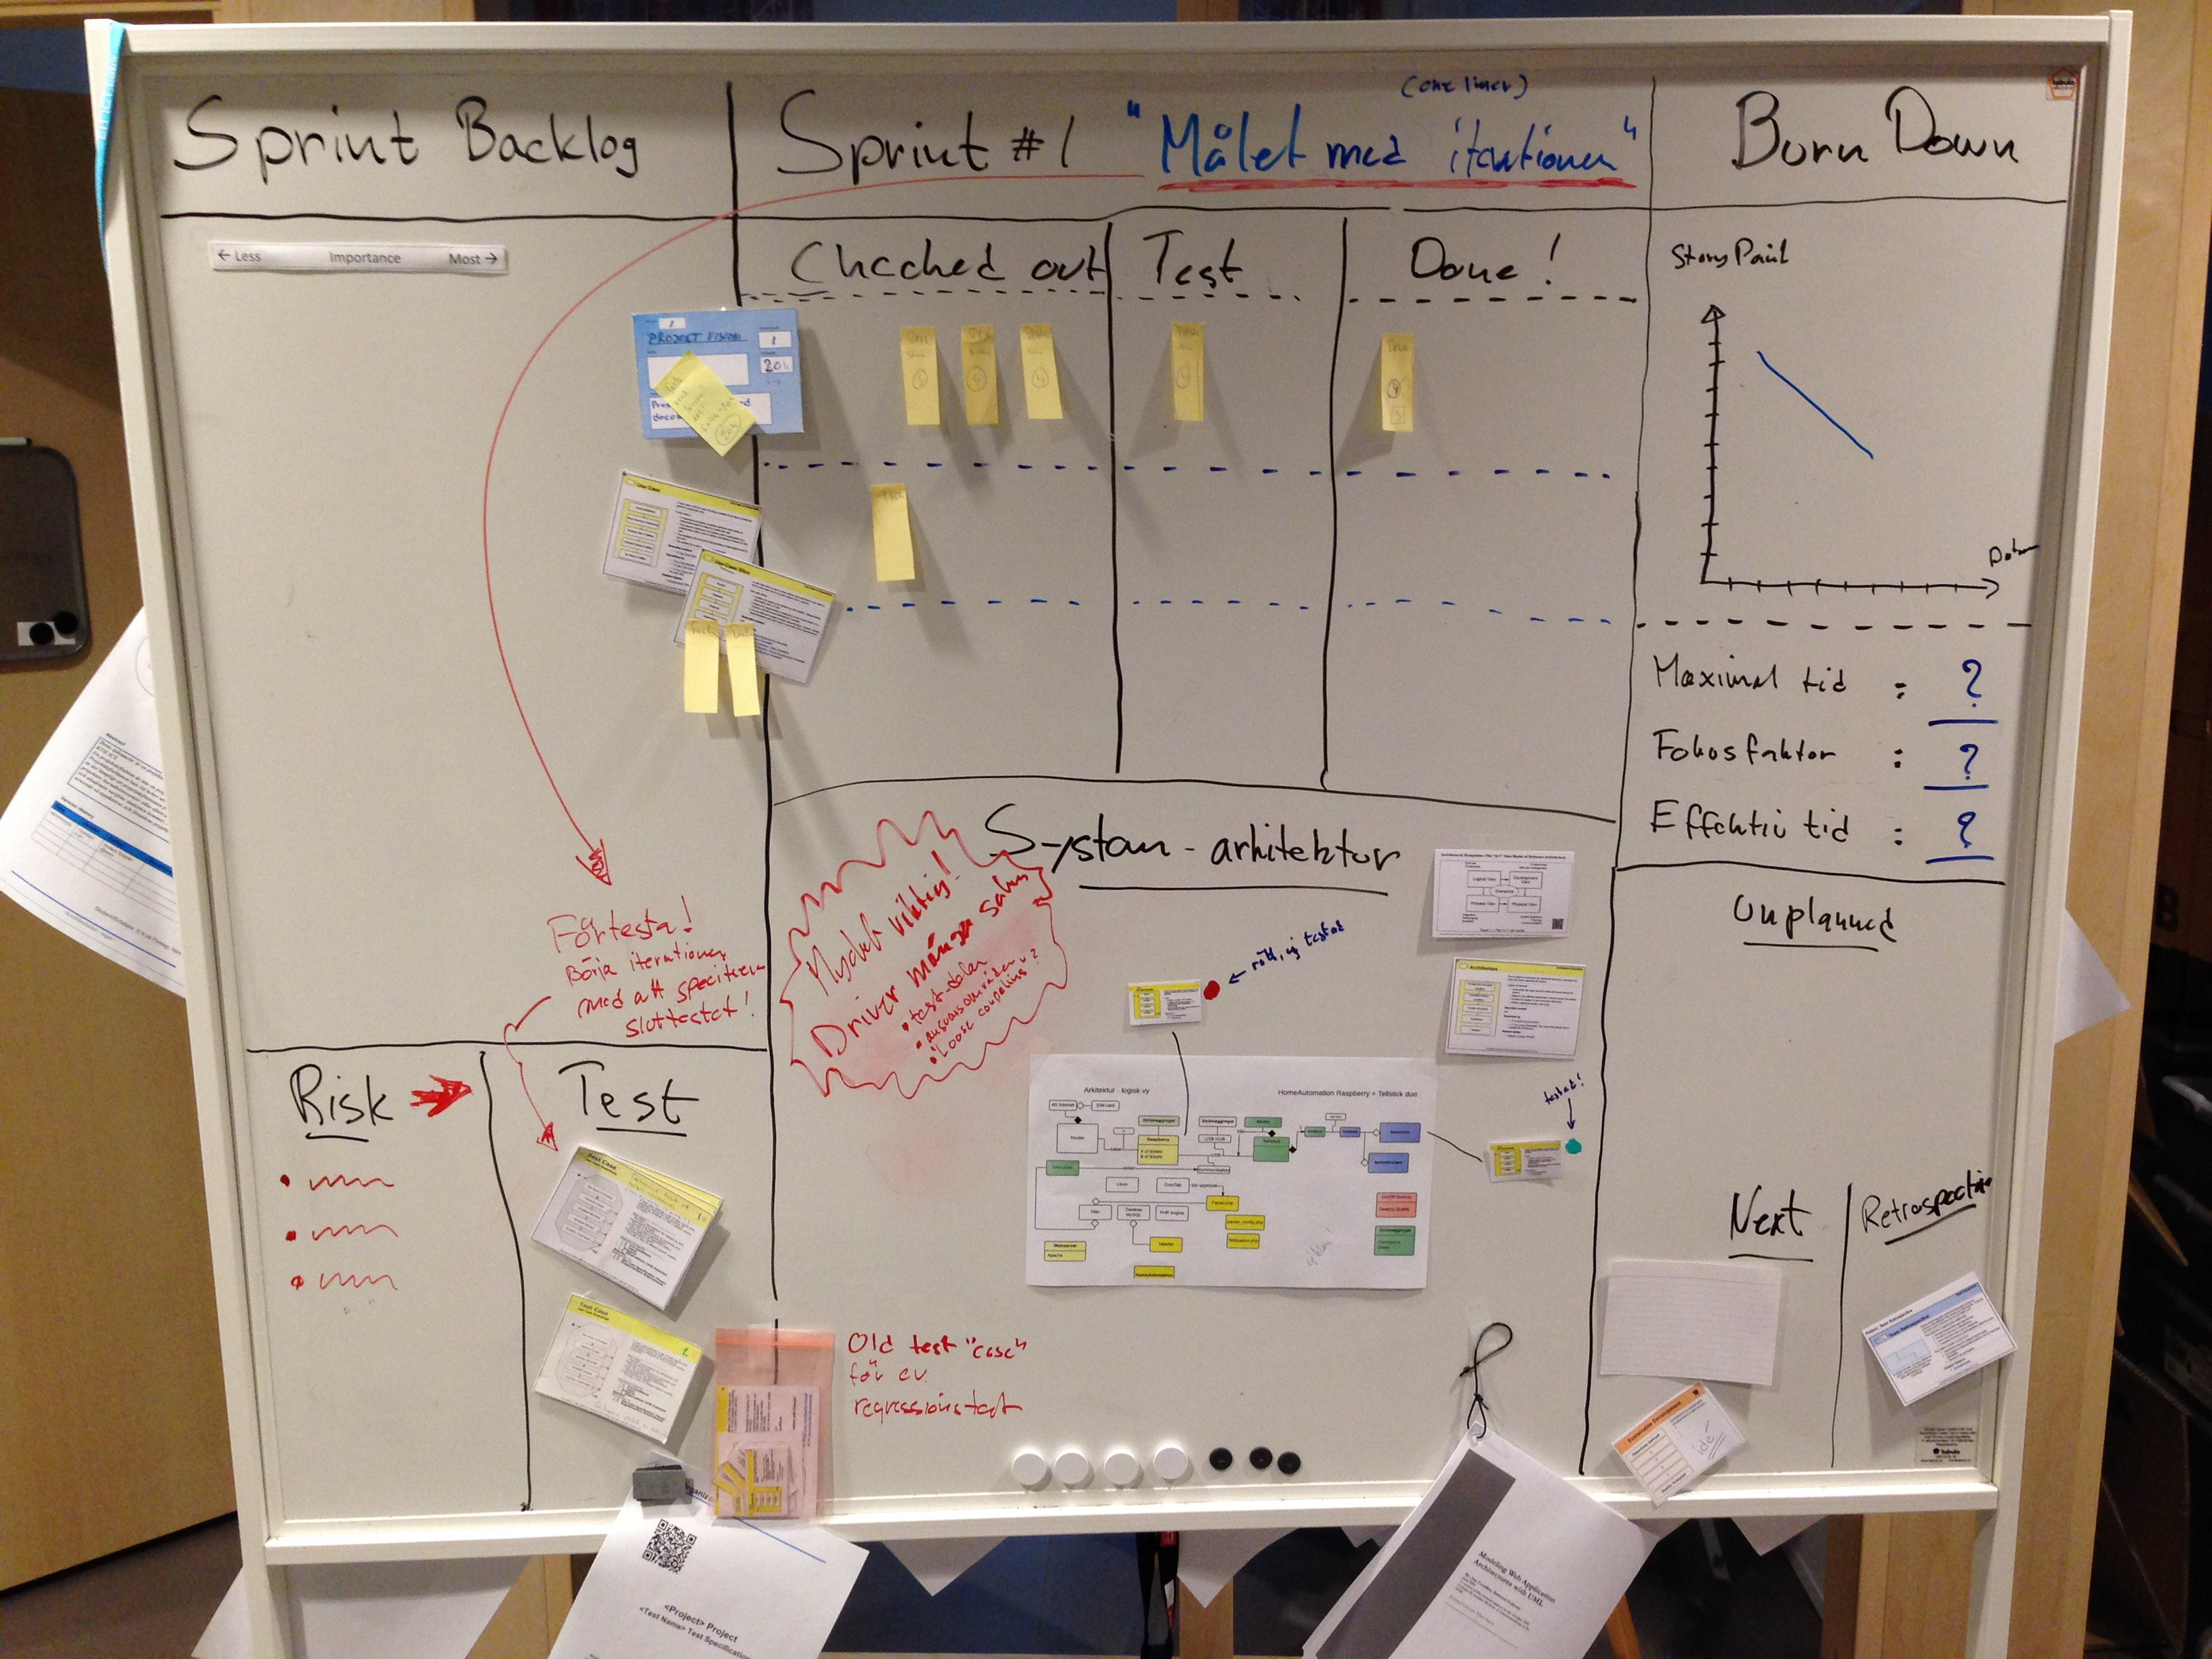
\includegraphics[width=3in]{sprintbacklog}
% where an .eps filename suffix will be assumed under latex, 
% and a .pdf suffix will be assumed for pdflatex; or what has been declared
\DeclareGraphicsExtensions.
\caption{Exempel på en intern sida för projektgruppen.}
\label{sprintbacklog}
\end{figure}

\begin{figure}[!ht]
\centering
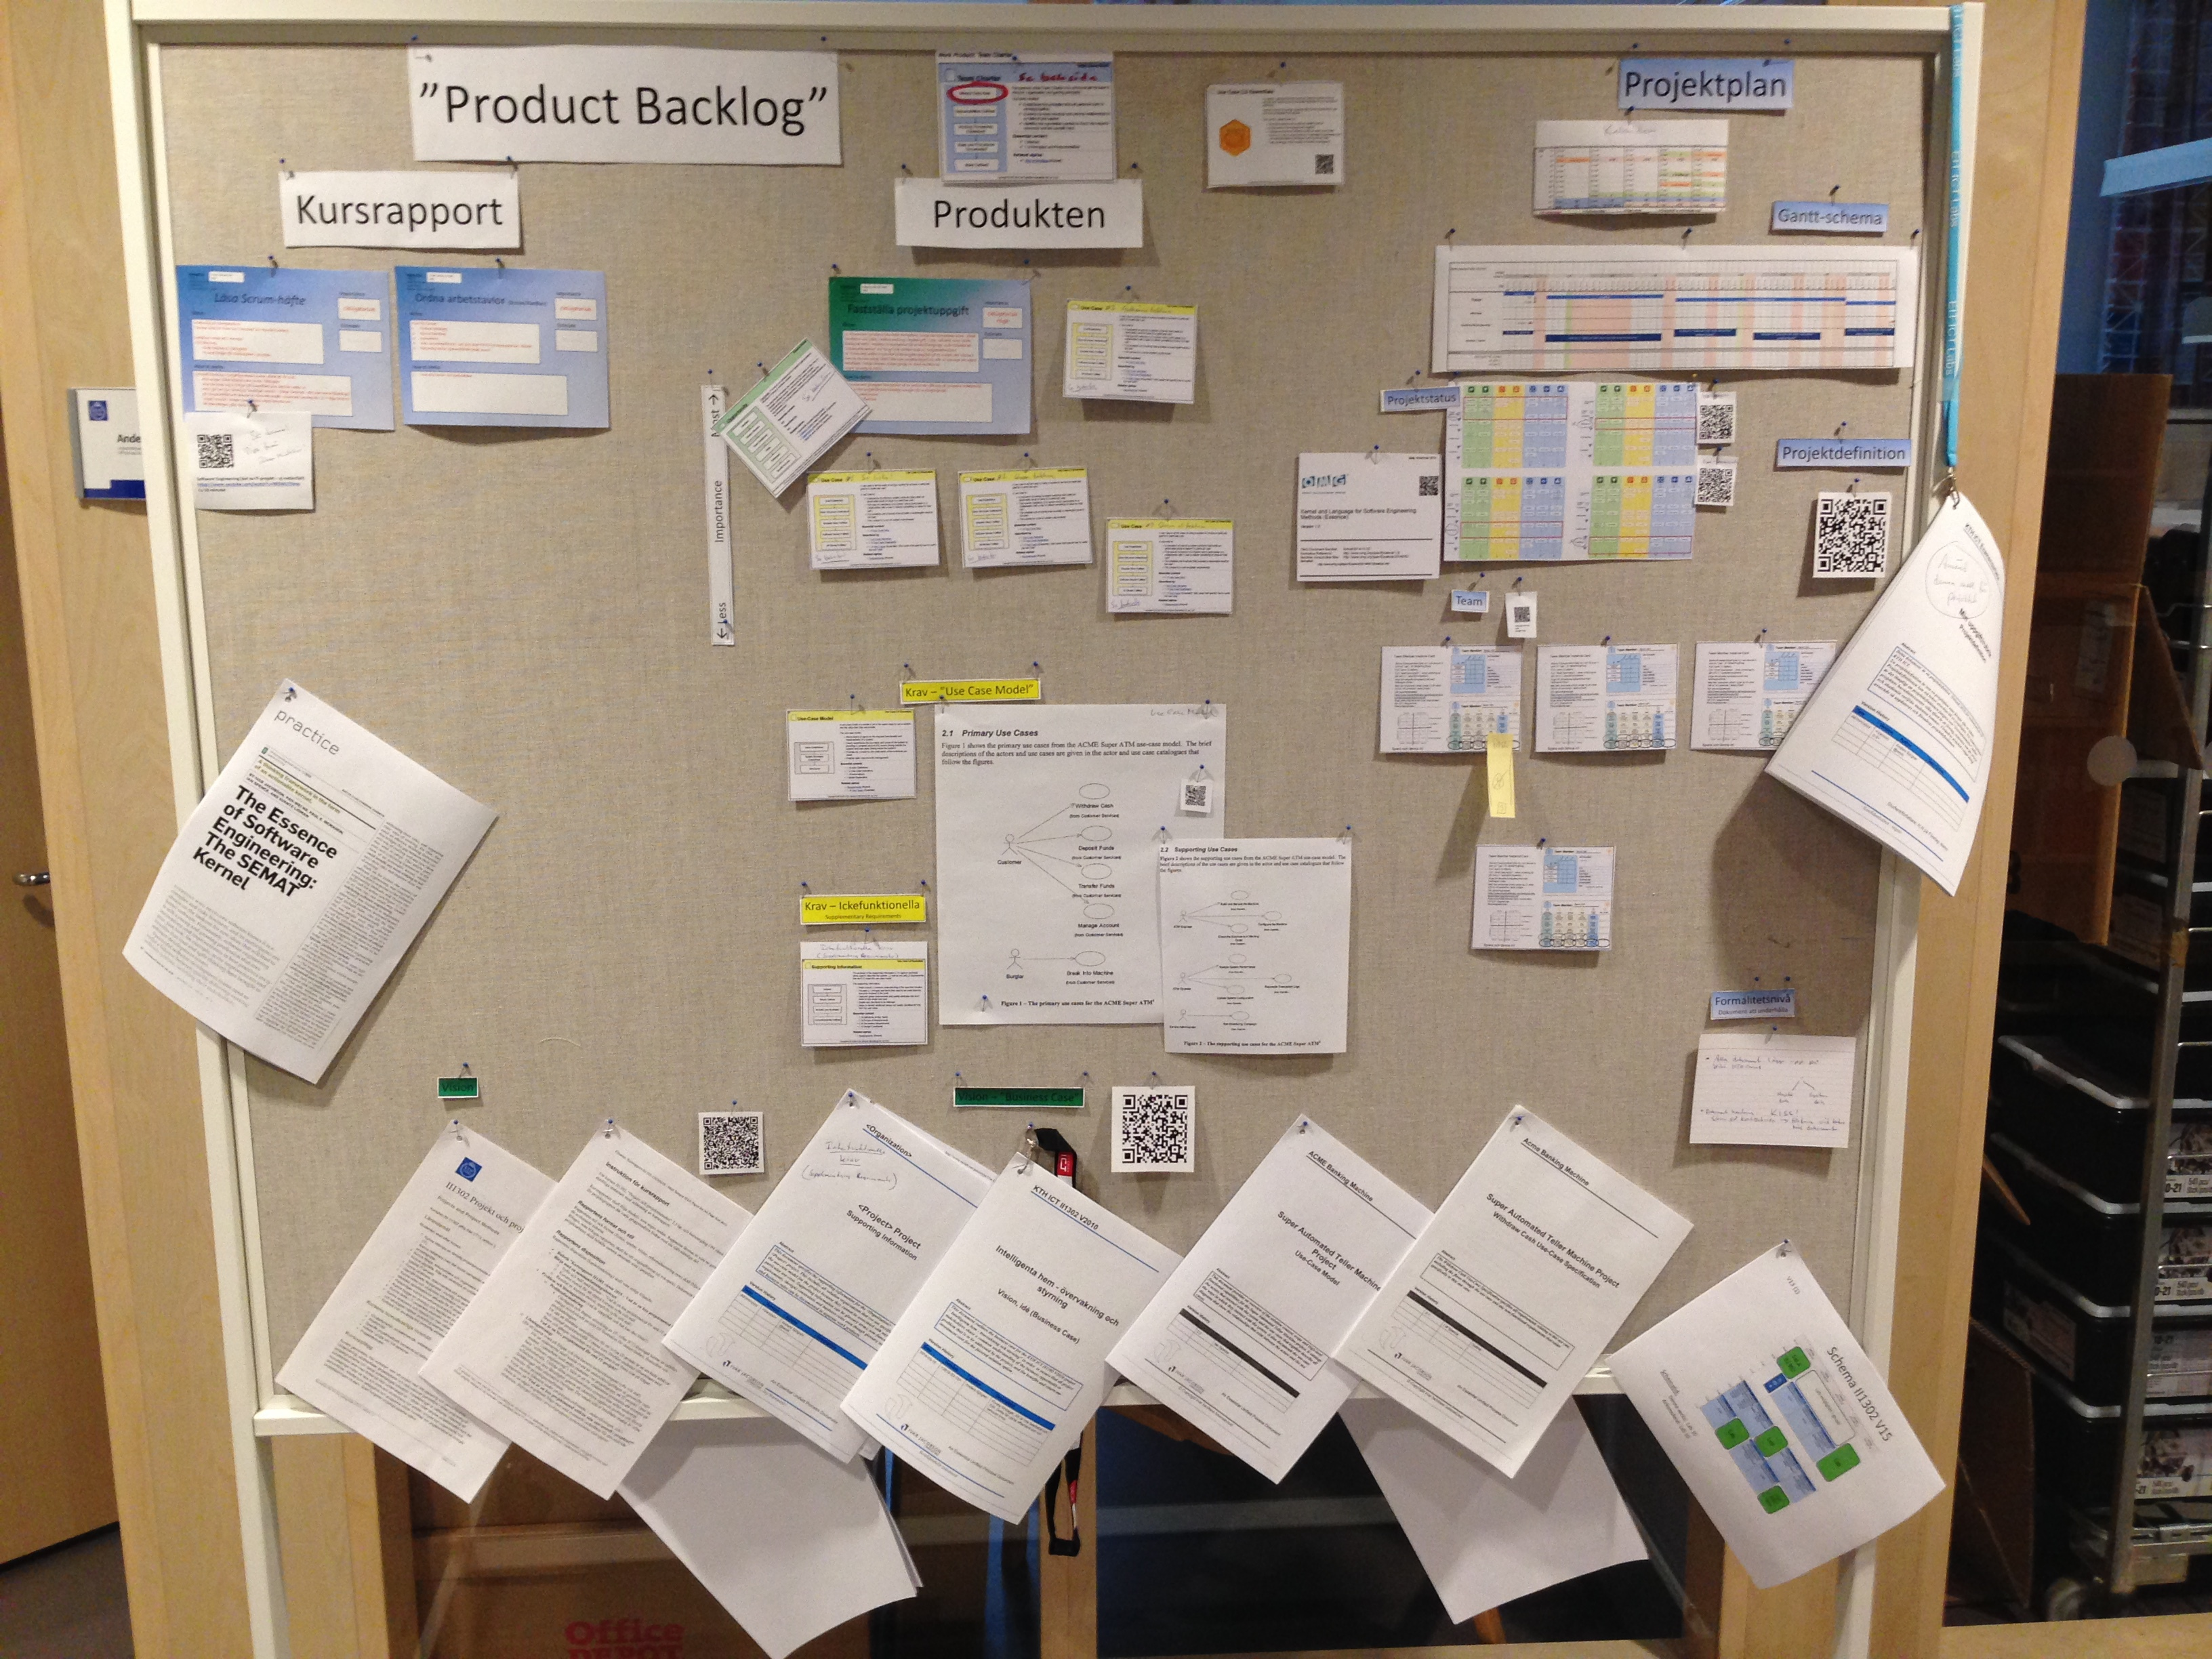
\includegraphics[width=3in]{productbacklog}
% where an .eps filename suffix will be assumed under latex, 
% and a .pdf suffix will be assumed for pdflatex; or what has been declared
\DeclareGraphicsExtensions.
\caption{Exempel på en public sida för projektgruppen.}
\label{productbacklog}
\end{figure}

\subsubsection{Scruminspirerade projektaktiviteter (vald ansats)}



% use section* for acknowledgment
\section{Undersökningsmetoder}
Detta kapitel beskriver vilka metoder som använts i undersökningen. Metoderna är valda och specificerade så att de skall kunna ge svar på ett antal följdfrågor som identifierats i denna undersökning. Först anges frågorna och sedan följer metodbeskrivning.
\subsection{Frågor att besvara i undersökningen}

\subsubsection{1}
\subsubsection{2}
\subsubsection{3}
\subsubsection{4}
\subsubsection{5}

\subsection{Metodbeskrivning}

\textbf{Metod 1: Undersökningsmetod}

%Exempel på hur man lägger in en bild
\begin{figure}[!ht]
\centering
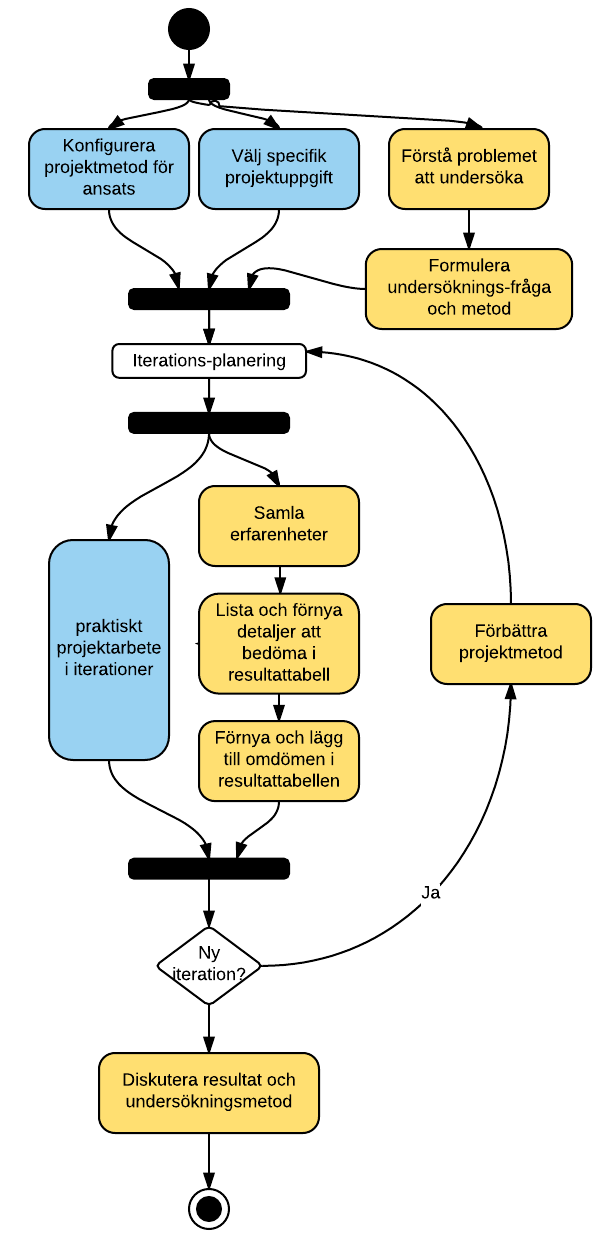
\includegraphics[width=2.5in]{invmethod}
% where an .eps filename suffix will be assumed under latex, 
% and a .pdf suffix will be assumed for pdflatex; or what has been declared
\DeclareGraphicsExtensions.
\caption{Undersökningsmetod för ``Vad är en bra projektmetod för små IT-projekt?''.}
\label{undersokningsmetod}
\end{figure}


\section{Genomförande}

\subsection{Projektledning}

\subsection{Kundrepresentant}

\section{Resultat}

% An example of a floating table. Note that, for IEEE style tables, the
% \caption command should come BEFORE the table and, given that table
% captions serve much like titles, are usually capitalized except for words
% such as a, an, and, as, at, but, by, for, in, nor, of, on, or, the, to
% and up, which are usually not capitalized unless they are the first or
% last word of the caption. Table text will default to \footnotesize as
% the IEEE normally uses this smaller font for tables.
% The \label must come after \caption as always.
%
%\begin{table}[!t]
%% increase table row spacing, adjust to taste
%\renewcommand{\arraystretch}{1.3}
% if using array.sty, it might be a good idea to tweak the value of
% \extrarowheight as needed to properly center the text within the cells
%\caption{An Example of a Table}
%\label{table_example}
%\centering
%% Some packages, such as MDW tools, offer better commands for making tables
%% than the plain LaTeX2e tabular which is used here.
%\begin{tabular}{|c||c|}
%\hline
%One & Two\\
%\hline
%Three & Four\\
%\hline
%\end{tabular}
%\end{table}
\section{Analys / Förbättringsförslag}

\section{Diskussion}

\subsection{Metoddiskussion}

\subsection{Resultatdiskussion}

\subsection{Bidrag till vetenskaplighet, ingenjörserfarenhet (studenterfarenhet?)}

\section{Slutord}

% trigger a \newpage just before the given reference
% number - used to balance the columns on the last page
% adjust value as needed - may need to be readjusted if
% the document is modified later
%\IEEEtriggeratref{8}
% The "triggered" command can be changed if desired:
%\IEEEtriggercmd{\enlargethispage{-5in}}

% references section

% can use a bibliography generated by BibTeX as a .bbl file
% BibTeX documentation can be easily obtained at:
% http://mirror.ctan.org/biblio/bibtex/contrib/doc/
% The IEEEtran BibTeX style support page is at:
% http://www.michaelshell.org/tex/ieeetran/bibtex/
%\bibliographystyle{IEEEtran}
% argument is your BibTeX string definitions and bibliography database(s)
%\bibliography{IEEEabrv,../bib/paper}
%
% <OR> manually copy in the resultant .bbl file
% set second argument of \begin to the number of references
% (used to reserve space for the reference number labels box)
%\begin{thebibliography}{1}

%\bibitem{IEEEhowto:kopka}
%H.~Kopka and P.~W. Daly, \emph{A Guide to \LaTeX}, 3rd~ed.\hskip 1em plus
%  0.5em minus 0.4em\relax Harlow, England: Addison-Wesley, 1999.

%\bibitem{}
  
%\end{thebibliography}

\nocite{*}
\bibliographystyle{IEEEtran}
\bibliography{sources}

% that's all folks
\end{document}


